% Day 7 notes, SC Quantathon v3 Bootcamp. Build: latexmk -pdf notes.tex
\documentclass[11pt]{article}

\usepackage[margin=1in]{geometry}
\usepackage{lmodern}
\usepackage[T1]{fontenc}
\usepackage{microtype}
\usepackage{amsmath,amssymb}
\usepackage{braket}
\usepackage{graphicx}
\usepackage{booktabs}
\usepackage{caption}
\usepackage{listings}
\usepackage{xcolor}
\usepackage[hidelinks]{hyperref}

\captionsetup{font=small,labelfont=bf}
\graphicspath{{figures/}}

\lstset{
  language=Python,
  basicstyle=\ttfamily\small,
  keywordstyle=\color{blue!60!black},
  commentstyle=\color{gray},
  stringstyle=\color{green!40!black},
  showstringspaces=false,
  frame=single,
  framerule=0.3pt,
  rulecolor=\color{gray!50},
  xleftmargin=1em,
  aboveskip=0.6em,
  belowskip=0.6em,
}

\newcommand{\code}[1]{\texttt{#1}}

\title{Day 7: Quantum Machine Learning}
\author{SC Quantathon v3 Bootcamp \\ Clemson Quantum Club}
\date{}

\begin{document}
\maketitle

\noindent
Quantum machine learning, in the form that runs today, is Day~6's variational loop pointed at data: a circuit that depends on an input $x$ and on trainable angles $\vec\theta$, an expectation value read off it, and a classical optimizer. These notes cover the two models that account for nearly all of it, the quantum kernel and the variational classifier, the encoding step both depend on, the gradient that trains the second, and the obstacle that limits both. They follow the order of the Day~7 notebook. Both datasets are synthetic and two-dimensional (Figure~\ref{fig:data}) so that every decision boundary can be drawn.

\begin{figure}[h]
\centering
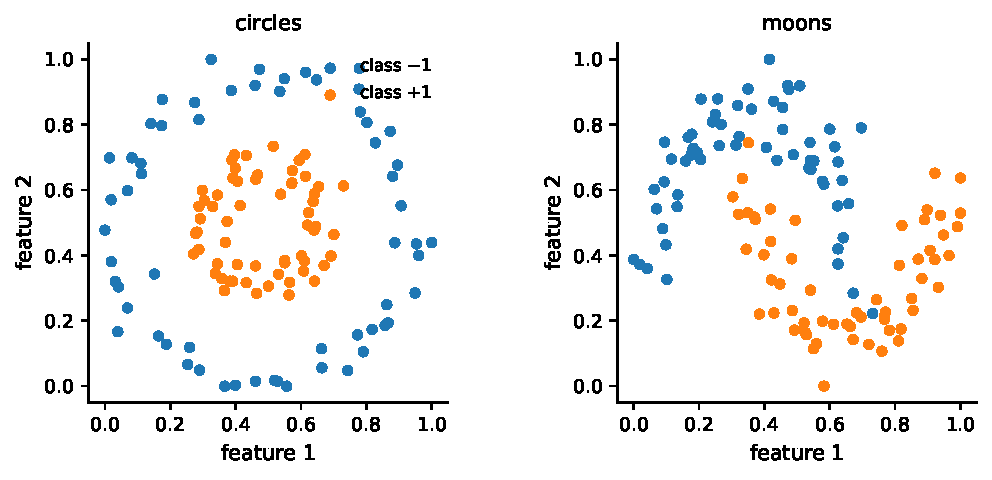
\includegraphics[width=0.8\textwidth]{datasets}
\caption{The two datasets, 120 points each, features scaled to $[0, 1]$: concentric circles and interleaved moons. Neither is separable by a straight line.}
\label{fig:data}
\end{figure}

\section{Encoding classical data into qubits}

A data point is a list of numbers; a qubit register is a state vector. The circuit that maps one to the other is the \emph{feature map} $U(x)$, and the state it prepares,
\begin{equation}
\ket{\phi(x)} = U(x)\ket{0\cdots0},
\label{eq:featuremap}
\end{equation}
is the only way the data ever enter a model. Three encodings cover most of what is used. \emph{Basis encoding} sends a bitstring to the basis state that spells it, one qubit per bit and no superposition. \emph{Angle encoding} sends each feature $x_i \in [0,1]$ to a rotation, $\ket{\phi(x)} = \bigotimes_i R_y(\pi x_i)\ket{0}$, one qubit per feature and a product state. \emph{Amplitude encoding} sends a vector of $2^n$ numbers, normalized, to the amplitudes of an $n$-qubit state: exponentially compact, but preparing a general such state costs a circuit of depth of order $2^n$. The notebook encodes $(3, 1, 2, 4)$ this way and reads back the probabilities $(0.300, 0.033, 0.133, 0.533)$, which are the squares of the normalized entries.

A product-state encoding can be simulated one feature at a time, so any kernel built from it is classically easy. Concretely, for the angle map the overlap factorizes: $\bra{0}R_y(\pi x_i)^\dagger R_y(\pi z_i)\ket{0} = \bra{0}R_y(\pi(z_i - x_i))\ket{0} = \cos\frac{\pi(z_i - x_i)}{2}$ on each qubit, so
\begin{equation}
k_{\rm angle}(x, z) = \prod_i \cos^2\frac{\pi(x_i - z_i)}{2},
\label{eq:anglekernel}
\end{equation}
a product of one factor per feature that a classical computer evaluates in time linear in the number of features, with no state vector anywhere. For the notebook's two test points, $(0.3, 0.8)$ and $(0.9, 0.1)$, Eq.~\eqref{eq:anglekernel} gives $0.071$, while the entangling map gives $0.105$: the CNOT and the product rotation have changed the geometry of the feature space, and no per-feature formula reproduces it. The maps used in practice add entangling gates and products of features. The notebook's \emph{entangling map} (Figure~\ref{fig:map}) encodes each feature as an $R_y$ angle, applies a CNOT, and then rotates the second qubit by $\pi x_0 x_1$, so the state depends on the features jointly. The \emph{ZZ feature map} of Havl\'i\v{c}ek et al.\ is the best-known alternative: $H$ on every qubit, a phase $2x_i$ on each, a phase $2(\pi - x_0)(\pi - x_1)$ on the pair through two CNOTs, the block repeated twice. Both are compared in the next section.

\begin{figure}[h]
\centering
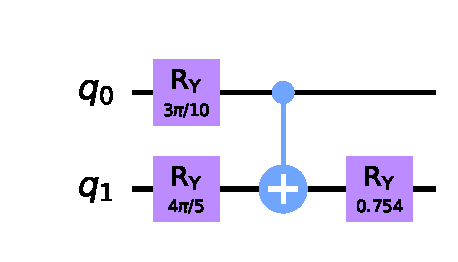
\includegraphics[width=0.5\textwidth]{feature_map}
\caption{The entangling map for the point $(0.3, 0.8)$.}
\label{fig:map}
\end{figure}

\section{Quantum kernels and the support vector machine}

Many classifiers use the data only through inner products between pairs of points. A \emph{kernel} $k(x, z)$ is such an inner product in some feature space, and a support vector machine (SVM) finds the boundary that separates the classes with the widest margin in that space, using only the kernel matrix $K_{ij} = k(x_i, x_j)$. A \emph{quantum kernel} is the overlap of two encoded states,
\begin{equation}
k(x, z) = \big|\braket{\phi(x)|\phi(z)}\big|^2 = \big|\braket{0|U(x)^\dagger U(z)|0}\big|^2 ,
\label{eq:kernel}
\end{equation}
which a processor estimates by running $U(x)^\dagger U(z)$ and counting how often all zeros comes back. Three properties make Eq.~\eqref{eq:kernel} a valid kernel. It is symmetric, and it equals 1 on the diagonal. And it is an inner product: $|\braket{a|b}|^2 = \operatorname{Tr}\big(\ket{a}\bra{a}\,\ket{b}\bra{b}\big)$, so $k$ is the inner product of the density matrices $\ket{\phi(x)}\bra{\phi(x)}$, and any matrix of inner products is positive semidefinite, which is what the SVM's optimization needs.

The SVM itself never sees the feature space. Its training problem depends on the data only through $K$, and its decision function is
\begin{equation}
f(x) = \sum_i \alpha_i\,y_i\,k(x, x_i) + b ,
\label{eq:svm}
\end{equation}
a weighted vote of the training points, with the weights $\alpha_i$ found by a convex optimization and nonzero only for the \emph{support vectors} that sit near the boundary. This is the \emph{kernel trick}: any feature map, including one into a $2^n$-dimensional Hilbert space, costs the same as long as its kernel can be evaluated. On hardware that cost is one circuit per pair, $N(N-1)/2 = 3160$ distinct circuits for the 80 training points and another $40\times80 = 3200$ for the test set, each needing enough shots to resolve overlaps near zero. Scikit-learn's \code{SVC(kernel="precomputed")} takes the training kernel matrix instead of raw features. Table~\ref{tab:svm} compares the quantum kernel SVM on both datasets with a linear SVM and an RBF-kernel SVM on the raw features, 80 training and 40 test points each; Figure~\ref{fig:svm} draws the decision regions.

\begin{table}[h]
\centering
\small
\begin{tabular}{@{}lllll@{}}
\toprule
dataset & quantum kernel, train & quantum kernel, test & linear SVM, test & RBF SVM, test \\
\midrule
circles & 100\% & 100\% & 52\% & 100\% \\
moons & 85\% & 90\% & 88\% & 100\% \\
\bottomrule
\end{tabular}
\caption{Test accuracy of the quantum kernel SVM with the entangling map against two classical baselines.}
\label{tab:svm}
\end{table}

\begin{figure}[h]
\centering
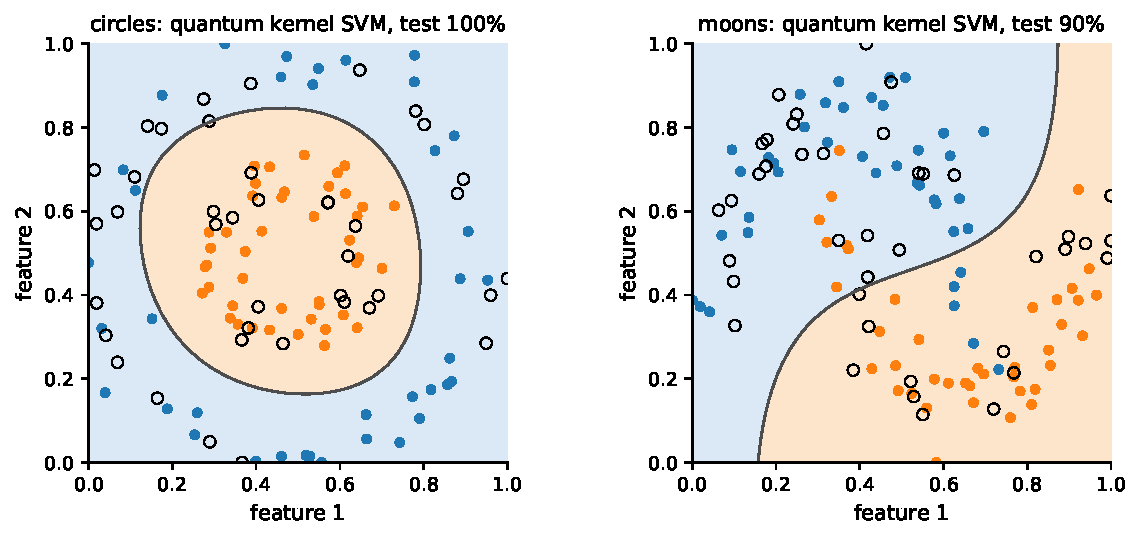
\includegraphics[width=0.95\textwidth]{kernel_svm}
\caption{Decision regions of the quantum kernel SVM. Filled points are training data, open circles are test data.}
\label{fig:svm}
\end{figure}

Two things follow from the table. The RBF baseline does at least as well, so on data like this the quantum kernel earns nothing beyond a demonstration; the argument for quantum kernels rests on feature maps whose overlaps are hard to compute classically, and on data with matching structure. And the feature map decides everything. The same SVM with the ZZ feature map scores 78\% on both datasets. Its pair phase $2(\pi - x_0)(\pi - x_1)$ runs from about 9 to 20 radians as the features cross $[0, 1]$, so two nearby points land on nearly orthogonal states and the kernel matrix loses the block structure the SVM needs (Figure~\ref{fig:matrices}): the entangling map's within-class blocks average 0.45 and 0.80 against the ZZ map's 0.39 and 0.74. Scaling the inputs by a factor $\beta < 1$ before encoding, the \emph{kernel bandwidth}, is the usual fix. In the other direction, as qubit count grows, random feature maps push all overlaps toward zero, a phenomenon called \emph{kernel concentration}, which makes $K$ close to the identity and the SVM useless. Feature maps have to be matched to the data, not just made deep.

\begin{figure}[h]
\centering
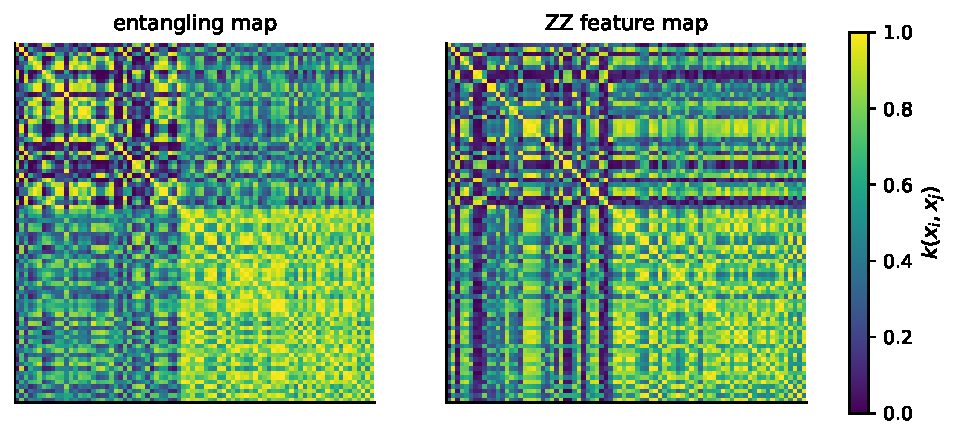
\includegraphics[width=0.85\textwidth]{kernel_matrices}
\caption{The $80\times80$ training kernel matrix of the circles data, rows and columns sorted by class, for the entangling map (left) and the ZZ feature map (right); the blocks are the two classes.}
\label{fig:matrices}
\end{figure}

\subsection{One kernel entry on the live machine}

The notebook's last section measures a single entry of Eq.~\eqref{eq:kernel} the way a processor has to: run $U(x)$ followed by $U(z)^\dagger$ and count how often \code{00} comes back. For the first two training points the exact overlap is $0.9206$; the simulator's 1000-shot estimate was $0.9250$ and the recorded run on \code{ibm\_kingston}, physical qubits 55 and 59, two \code{cz} gates at depth 13, gave $0.9290$ (929 of \code{00}, 65 of \code{01}, 2 of \code{10}, 4 of \code{11}). At $p \approx 0.92$ and 1000 shots the shot noise alone is $\sqrt{p(1-p)/N} \approx 0.009$, so both estimates sit within one standard deviation of the exact value, and this entry says nothing about gate error. That is expected: a percent of two-qubit gate error shifts $P(\code{00})$ by less than a percent, below the shot noise of a 1000-shot estimate, and the recorded value even sits above the exact one, the opposite direction from what depolarizing noise pushes. Gate error shows itself on entries near 0, which noise lifts away from zero and which a kernel matrix has many more of than entries near 1. Estimating a full $80\times80$ matrix to that precision is 3160 circuits at a thousand shots each, the cost quoted above.

\section{A variational quantum classifier}

The second model replaces the SVM with a trainable circuit. Encode $x$ with the feature map, apply the hardware-efficient ansatz $W(\vec\theta)$ of Day~6 (two qubits, two entangling layers, six angles), and read one expectation value,
\begin{equation}
f(x;\vec\theta) = \braket{\phi(x)|\,W(\vec\theta)^\dagger\, Z_0\, W(\vec\theta)\,|\phi(x)} \in [-1, 1],
\label{eq:vqc}
\end{equation}
whose sign is the predicted class (Figure~\ref{fig:vqccircuit}). Any observable with eigenvalues $\pm1$ would serve; $Z_0$ is the cheapest, one qubit read in the computational basis, and the parity $Z_0Z_1$ is the usual alternative. There is no bias term, so the boundary is wherever $f$ crosses zero; shifting that threshold is a one-parameter classical afterthought that the notebook leaves out. Training chooses $\vec\theta$ to make $f$ close to the labels $y_i \in \{-1, +1\}$ under the squared-error loss
\begin{equation}
L(\vec\theta) = \frac{1}{N}\sum_{i=1}^{N}\big(f(x_i;\vec\theta) - y_i\big)^2 .
\label{eq:loss}
\end{equation}
Every input and every angle is a circuit parameter, so one parameterized circuit and one Estimator call evaluate $f$ on the whole dataset. At the notebook's random starting angles the loss is 2.0; a model that outputs $f = 0$ everywhere has loss exactly 1, so a random start can be worse than saying nothing.

\begin{figure}[h]
\centering
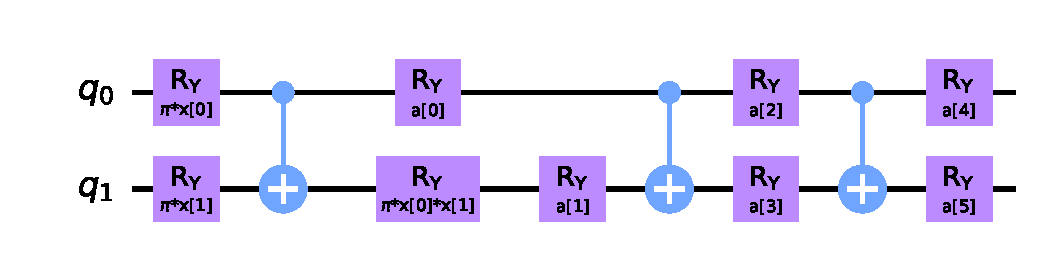
\includegraphics[width=0.95\textwidth]{vqc_circuit}
\caption{The classifier circuit: the entangling map with symbolic inputs $x_0, x_1$, followed by the six-angle ansatz. The observable is $Z$ on qubit 0.}
\label{fig:vqccircuit}
\end{figure}

\section{Gradients and training}

Every trainable gate is $R_y(\theta_k) = e^{-i\theta_k Y/2}$, so $f$ is a sinusoid in each angle, $a + b\cos\theta_k + c\sin\theta_k$, exactly as for the energy on Day~6, and its derivative is the \emph{parameter-shift rule}
\begin{equation}
\frac{\partial f}{\partial\theta_k} = \frac12\Big[f\big(\theta_k + \tfrac\pi2\big) - f\big(\theta_k - \tfrac\pi2\big)\Big] .
\label{eq:shift}
\end{equation}
Exact, not a finite difference, and made of ordinary circuit runs. Because $f$ is a sinusoid of amplitude at most 1 in each angle, every component of its gradient is bounded by 1, and the loss landscape repeats with period $2\pi$ in every direction, so no learning rate can send an angle to infinity, only around the circle. The notebook checks the rule against a finite difference with step $10^{-5}$ and the two agree to $5\times10^{-11}$. The chain rule then gives the loss gradient,
\begin{equation}
\frac{\partial L}{\partial\theta_k} = \frac{2}{N}\sum_{i=1}^N \big(f(x_i;\vec\theta) - y_i\big)\,\frac{\partial f(x_i;\vec\theta)}{\partial\theta_k} ,
\label{eq:lossgrad}
\end{equation}
which costs $2P$ evaluations of the model, each an Estimator call over all $N$ points, for $P$ angles. Gradient descent, $\vec\theta \leftarrow \vec\theta - \eta\,\nabla L$ with $\eta = 0.4$ for 60 steps and the best of three random starts, brings the loss on the circles data from 0.64 after the first step to 0.44 and the training accuracy to 90\%; all three starts end at the same loss, and the held-out accuracy is 78\% (Figure~\ref{fig:vqc}). A six-angle circuit is a small model, and it draws a smooth closed curve around the inner class rather than the sharp ring of the kernel SVM. On hardware a single gradient step is $2PN$ circuit jobs before shot noise is considered, and that cost, not the mathematics, is what limits variational classifiers today.

\begin{figure}[h]
\centering
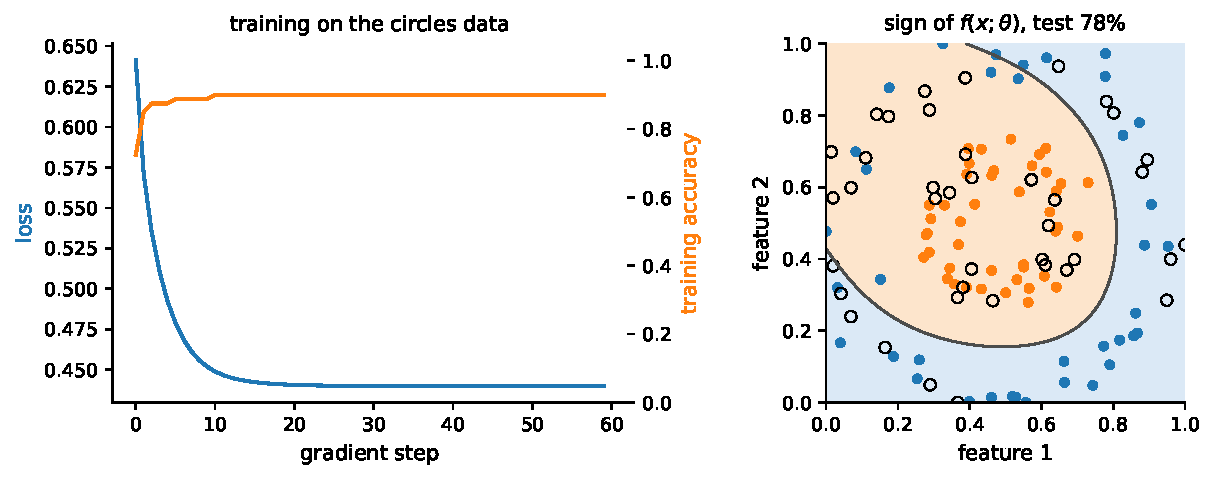
\includegraphics[width=0.98\textwidth]{vqc}
\caption{Left: loss and training accuracy over 60 gradient steps on the circles data. Right: the sign of $f(x;\vec\theta)$ after training, with training points filled and test points open.}
\label{fig:vqc}
\end{figure}

\section{Barren plateaus}

Make the ansatz wider and deeper and something goes wrong that no optimizer can fix. For random angles in a sufficiently deep circuit, the gradient of any expectation value is zero on average and its \emph{variance shrinks exponentially with the number of qubits}: for circuits deep enough to scramble the state like a random unitary, McClean et al.\ showed the variance is of order $2^{-n}$ for a Pauli observable. The number comes from averaging over random states. For a state drawn uniformly from the $d = 2^n$-dimensional Hilbert space, the expectation value of a traceless observable $H$ with $H^2 = I$ has mean zero and
\begin{equation}
\operatorname{Var}\big[\braket{\psi|H|\psi}\big] = \frac{\operatorname{Tr}H^2}{d(d+1)} = \frac{1}{2^n + 1},
\label{eq:haar}
\end{equation}
since $\operatorname{Tr}H^2 = d$. A parameter-shift gradient is half the difference of two such expectation values, so its variance is of the same order, and it halves with every added qubit. A landscape whose slopes are exponentially small everywhere cannot be climbed from a random start, since even the direction of the first step is lost in shot noise. The notebook measures this directly: a hardware-efficient ansatz with as many entangling layers as qubits, a hundred random parameter settings, and the parameter-shift derivative of $\braket{Z_0Z_1}$ with respect to the first angle (Table~\ref{tab:bp}, Figure~\ref{fig:bp}).

\begin{table}[h]
\centering
\small
\begin{tabular}{@{}lllllll@{}}
\toprule
qubits $n$ & 2 & 3 & 4 & 5 & 6 & 8 \\
\midrule
$\operatorname{Var}[\partial_{\theta_1}\braket{Z_0Z_1}]$ & $0.233$ & $0.102$ & $0.073$ & $0.038$ & $0.026$ & $0.013$ \\
\bottomrule
\end{tabular}
\caption{Variance of one gradient component over 100 random parameter settings, for an ansatz with $n$ qubits and $n$ entangling layers.}
\label{tab:bp}
\end{table}

\begin{figure}[h]
\centering
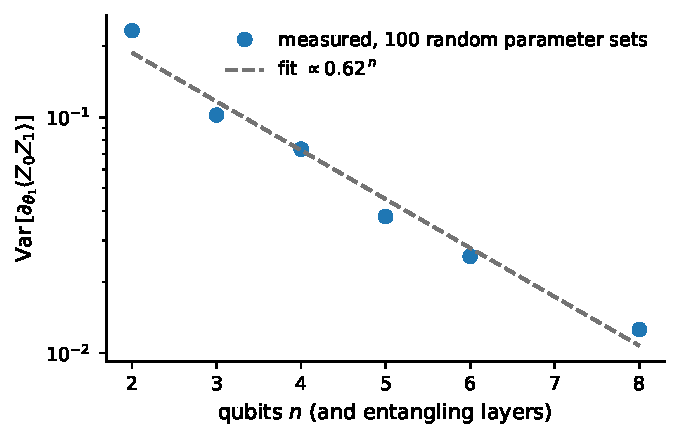
\includegraphics[width=0.58\textwidth]{barren_plateau}
\caption{The variance of Table~\ref{tab:bp} on a log scale, with an exponential fit.}
\label{fig:bp}
\end{figure}

The straight line on the log axis is the exponential: a factor of 0.62 per added qubit over this range, a factor of about 18 between 2 and 8 qubits. Eq.~\eqref{eq:haar} sets the scale a fully scrambling circuit would reach: $0.200$, $0.111$, $0.059$, $0.030$, $0.015$, and $0.004$ for the six widths, for the expectation value itself; the gradient, half a difference of two such values, is of the same order. From four qubits on the measured variances sit above that scale, and the gap widens with width, because $n$ entangling layers on $n$ qubits is not yet deep enough to scramble the state completely. Deeper circuits approach the $1/(2^n+1)$ line, and the plateau only gets flatter. The ways around it are an active research area: shallow circuits, ansätze built from the problem rather than from convenience (Day~6's one-parameter ansatz is the model case), initializing near the identity, and structured feature maps. They all amount to not searching the whole exponentially large space at once.

\section{What transfers to the hackathon}

\begin{itemize}
\item Fit the classical baselines first. A linear model, an RBF SVM, and a small tree ensemble take minutes and set the bar a quantum model has to clear; a result that does not beat them is not a result.
\item Count features. A quantum model needs one qubit per feature for angle encoding and $\log_2$ of the count for amplitude encoding; a dataset with fifty columns has to be reduced, by principal components or by choosing columns, before it fits.
\item Split and cross-validate. Report held-out accuracy, and repeat over several splits, since with 40 test points one point is 2.5\%. Scale the features with statistics of the training set only and apply the same transformation to the test set; fitting the scaler on everything leaks the test data into the model.
\item Watch the kernel matrix. If it is close to the identity, the map is too wide or too deep for the data (kernel concentration); if it is nearly all ones, the map is too narrow. Scale the inputs until the blocks appear.
\item Budget shots. A kernel matrix for $N$ training points is $N(N-1)/2$ circuits on hardware, each needing enough shots to resolve overlaps near zero; a variational classifier is $2PN$ circuits per gradient step. Simulate first and go to hardware for one confirming run.
\end{itemize}

\section{Summary}

\begin{itemize}
\item A feature map $U(x)$ turns data into a state, Eq.~\eqref{eq:featuremap}. Basis, angle, and amplitude encoding are the basic choices; entangling maps are what give quantum models a feature space a product state does not have.
\item A quantum kernel is the overlap of two encoded states, Eq.~\eqref{eq:kernel}: symmetric, unit diagonal, positive semidefinite. With an SVM it separates the circles and moons data (Table~\ref{tab:svm}); an RBF kernel does as well, and the map's bandwidth decides whether the kernel carries structure at all.
\item A variational classifier reads the sign of an expectation value, Eq.~\eqref{eq:vqc}, and is trained on the squared loss, Eq.~\eqref{eq:loss}, with parameter-shift gradients, Eqs.~\eqref{eq:shift} and~\eqref{eq:lossgrad}. Six angles reach 90\% training accuracy on the circles data.
\item The variance of a gradient component falls exponentially with qubit count in deep random circuits, a barren plateau (Table~\ref{tab:bp}); shallow, problem-shaped circuits and careful initialization are the ways around it.
\item One kernel entry measured on a processor landed within shot noise of the exact overlap; the cost of a whole matrix, thousands of such circuits, is the real constraint.
\item Classical baselines, feature counts, held-out evaluation, the kernel matrix, and shot budgets decide whether a quantum model is worth running on a hackathon dataset.
\end{itemize}

\begin{thebibliography}{9}
\bibitem{havlicek} V.~Havl\'i\v{c}ek et al., ``Supervised learning with quantum-enhanced feature spaces,'' Nature \textbf{567}, 209 (2019). The ZZ feature map and the quantum kernel SVM.
\bibitem{schuldkilloran} M.~Schuld and N.~Killoran, ``Quantum machine learning in feature Hilbert spaces,'' Phys. Rev. Lett. \textbf{122}, 040504 (2019). Feature maps as kernels.
\bibitem{mitarai} K.~Mitarai, M.~Negoro, M.~Kitagawa, and K.~Fujii, ``Quantum circuit learning,'' Phys. Rev. A \textbf{98}, 032309 (2018). The variational classifier and the parameter-shift rule.
\bibitem{mcclean} J.~R. McClean, S.~Boixo, V.~N. Smelyanskiy, R.~Babbush, and H.~Neven, ``Barren plateaus in quantum neural network training landscapes,'' Nature Communications \textbf{9}, 4812 (2018).
\bibitem{shaydulin} R.~Shaydulin and S.~M. Wild, ``Importance of kernel bandwidth in quantum machine learning,'' Phys. Rev. A \textbf{106}, 042407 (2022).
\bibitem{cerezo} M.~Cerezo et al., ``Variational quantum algorithms,'' Nature Reviews Physics \textbf{3}, 625 (2021). A review of the whole family.
\bibitem{ibmqml} IBM Quantum Learning, \emph{Quantum machine learning}. \url{https://quantum.cloud.ibm.com/learning/en/courses/quantum-machine-learning}
\end{thebibliography}

\end{document}
